% Magic comments - Informa ao compilador algumas regras de execução, como tipo de compilação ou codificação do texto
% !TeX encoding = UTF-8
% !BIB TS-program = XeLaTex
% !TeX root = slides-oficina-latex-pos-letras-2019.tex
% !TeX encoding = UTF-8
% !BIB TS-program = XeLaTex
% !backend = biber

%% This work may be distributed and/or modified under the
%% conditions of the LaTeX Project Public License, either version 1.3
%% of this license or (at your option) any later version.
%% The latest version of this license is in
%%   http://www.latex-project.org/lppl.txt
%% and version 1.3 or later is part of all distributions of LaTeX
%% version 2005/12/01 or later.
%%
%% This work consists of the files slides-oficina-latex-pos-letras-2019.tex, 
%%
%% Modelo adaptado por Danny A. V. Tonidandel (tonidandel@gmail.com), a partir do template de Fábio Rodrigues Silva (gfabinhomat@gmail.com)
%% Mais informações podem ser obtidas no guia do usuário Beamer 
%% (http://linorg.usp.br/CTAN/macros/latex/contrib/beamer/doc/beameruserguide.pdf)
%% Informações rápidas podem ser acessadas em http://en.wikibooks.org/wiki/LaTeX/Presentations
%%
%% Alterações feitas: 
%% 1) Cores do sistema, sobretudo na página de título, com logos das instituições;
%% 2) pacotes para compilação a partir do XeLaTeX e bibliografias reduzidas (ibid., op.cit. etc.) em notas de rodapé, estilo biblatex-abnt-ibid ou estilo abnt com notas explicativas;
%% 3) Algumas adequações para atender à norma ABNT NBR6023-2018.


% Apresentações em widescreen. Outros valores possíveis: 1610, 149, 54, 43 e 32.
% Por padrão, as apresentações são no formato 4:3 (sem o aspectratio).
\documentclass[aspectratio=169]{beamer}	 	

\usetheme{Pittsburgh}
\usecolortheme{default}
\usefonttheme[onlymath]{serif}			% para fontes matemáticas
% Enconte mais temas e cores em http://www.hartwork.org/beamer-theme-matrix/ 
% Veja também http://deic.uab.es/~iblanes/beamer_gallery/index.html

% Customizações de Cores: fg significa cor do texto e bg é cor do fundo
\definecolor{coolblack}{rgb}{0.0, 0.18, 0.39} % define cor coolblack
\definecolor{cornellred}{rgb}{0.7, 0.11, 0.11} % define cor cornellred
\definecolor{darkelectricblue}{rgb}{0.33, 0.41, 0.47} % define cor darkelectricblue
%% Para definir mais cores, visite https://latexcolor.com/
\setbeamercolor{normal text}{fg=black}
\setbeamercolor{alerted text}{fg=cornellred}
\setbeamercolor{author}{fg=cornellred}
\setbeamercolor{institute}{fg=coolblack}
\setbeamercolor{date}{fg=darkelectricblue}
\setbeamercolor{frametitle}{fg=coolblack}
\setbeamercolor{framesubtitle}{fg=cornellred}
\setbeamercolor{block title}{bg=darkelectricblue, fg=white}		%Cor do título
\setbeamercolor{block body}{bg=lightgray, fg=darkgray}	%Cor do texto (bg= fundo; fg=texto)
%--

% ---
% PACOTES
% ---
\usepackage[backend=biber,
style=abnt-ibid,
citecount,
ittitles,
giveninits,
scbib,
justify,
noslsn,
repeatfields]{biblatex} % Citações padrão ABNT com estilo biblatex-abnt

\addbibresource{referencias.bib}
\usepackage{relsize} % precisa ser readicionado por que senão o comando \part não funciona no biblatex.  
\usepackage[brazil]{babel}		% Idioma do documento em português
\usepackage{color}			% Controle das cores
\usepackage{amsmath,amssymb,unicode-math} % segundo informacoes, o pacote unicode-math é mais adequado para o compilador xelatex, ao invés do amsfonts
%\usepackage[T1]{fontenc}		% Selecao de codigos de fonte.
\usepackage{graphicx}			% Inclusão de gráficos
%\usepackage[utf8]{inputenc}		% Codificacao do documento (conversão automática dos acentos)
%\usepackage{txfonts}			% Fontes virtuais
\usepackage[style=brazilian]{csquotes}
\usepackage{fourier-orns} % decoracoes 

% --- Adequacao ao estilo abnt (2018) - formata campo url
\DeclareFieldFormat{url}{\bibstring{urlfrom}\addcolon\addspace \url{#1}}%

% --- Informações do documento ---
\title{Um título interessante}
\author{\aldineleft Clarice Lispector }
\institute{Dissertação (mestrado)
	\par
	Orientador: Profa. Mary B. Hesse, PhD.
	    \par
	    Coorientador: Prof. Thomas Kuhn, PhD. 
    	}
    
\date{\small{\today}}
% ---

% ----------------- INÍCIO DO DOCUMENTO --------------------------------------
\begin{document}

% ----------------- NOVO SLIDE -- CAPA --------------------------------
\begin{frame}

\begin{minipage}{1\linewidth}
  \centering
  \begin{tabular}{ccc}
    \begin{tabular}{c}
    	
\includegraphics[scale=0.3]{figuras/logo-ichs.pdf}
    \end{tabular}
    &
    \begin{tabular}{c}
      \textbf{Universidade Federal de Ouro Preto} \\ \textbf{Programa de Pós-Graduação em Letras: estudos da Linguagem}
    \end{tabular}
	&
  \begin{tabular}{c}
	      
\includegraphics[scale=0.8]{figuras/logo-ufop.pdf} 
\end{tabular}
  \end{tabular}
\end{minipage}
\titlepage % imprime dados como título e autor
\end{frame}

% ----------------- NOVO SLIDE --------------------------------
\begin{frame}{Sumário}
\tableofcontents
\end{frame}

% ----------------- NOVO SLIDE --------------------------------
\section{Uma introdução}

% ----------------- NOVO SLIDE --------------------------------

\begin{frame}{Pra começar a história...}
\begin{minipage}{0.4\textwidth}
	\begin{figure}
		\centering
		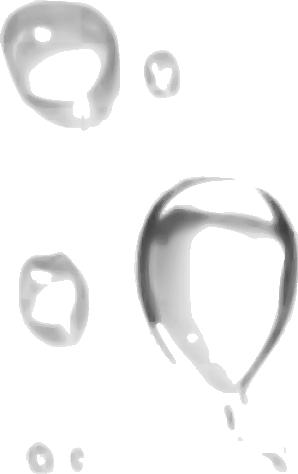
\includegraphics[scale=0.2]{figuras/gota-dagua.pdf}
	\end{figure}
\end{minipage}
%\begin{minipage}{0.57\textwidth}
\begin{itemize}
	\item Antes de Bauman, Descartes já dizia: ``o mundo é líquido'';\footcite{descartes-metodo}
	\item Em outro techo da obra, Descartes faz afirmação semelhante \footcite[O que pode ser visto no segundo capítulo. Ver, por exemplo,][p.~56]{descartes-metodo}
	\item ``Samosata foi o primeiro a contar a história do espelho de Arquimedes;''\footcite{luciano-de-samosata}
\end{itemize}
%\end{minipage}
\end{frame}
% ----------------- NOVO SLIDE --------------------------------


% ----------------- NOVO SLIDE --------------------------------
\section{Metodologia e Organização}
% ----------------- NOVO SLIDE --------------------------------
\begin{frame}{Um símbolo impactante}
\framesubtitle{Uma fala inicial...}
Um texto e uma figura...
\begin{figure}
	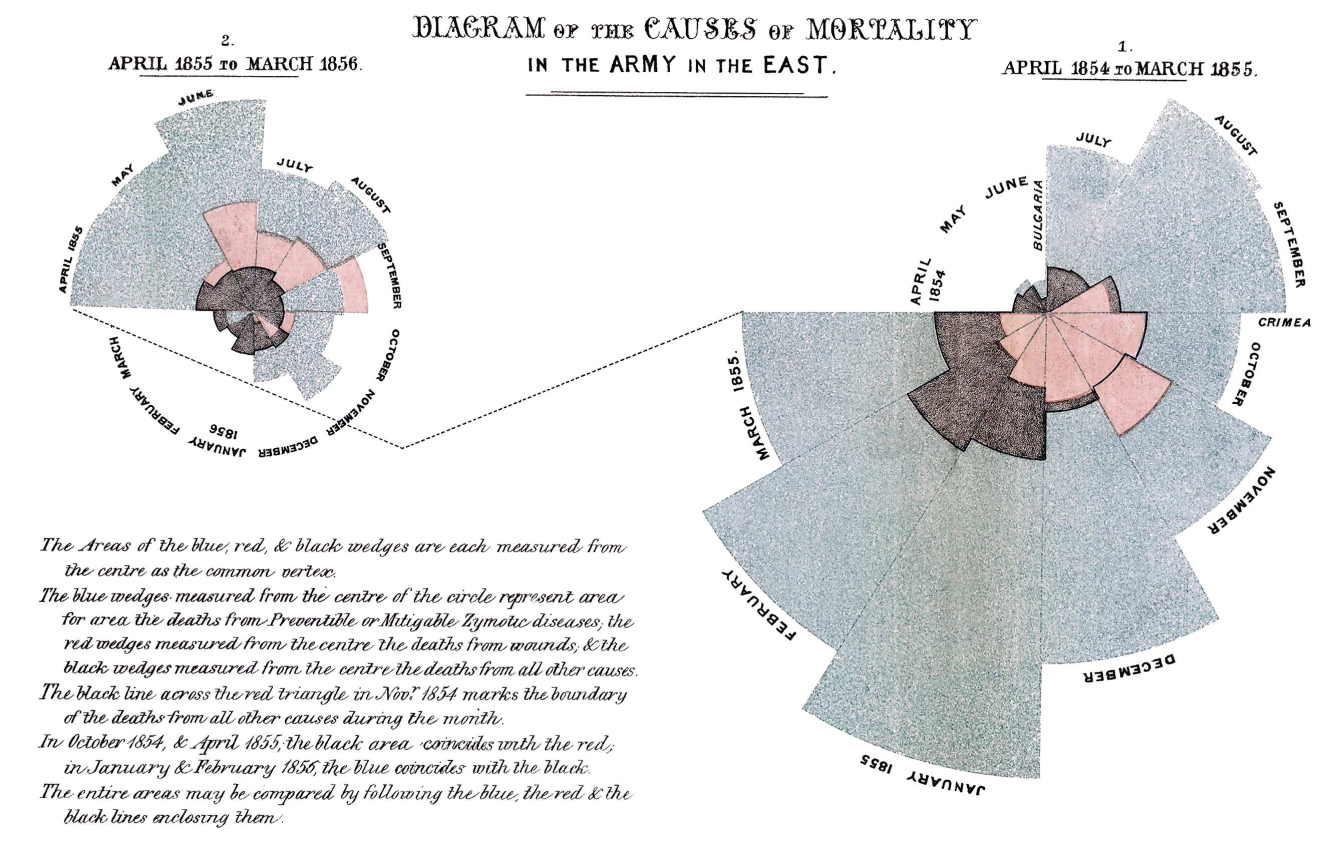
\includegraphics[scale=0.6]{figuras/rose-diagram.png}
	\caption{O diagrama polar de Florence Nightingale (1854). Disponível em: \url{http://bit.ly/2MBkXkk}.}
\end{figure}
\end{frame}
% ----------------- NOVO SLIDE --------------------------------

% ----------------- NOVO SLIDE --------------------------------
\begin{frame}{Duo figuras}
\begin{minipage}{0.47\textwidth}
\begin{figure}[hbtp]
	\centering
	
\includegraphics[scale=0.3]{figuras/abntex2-modelo-img-marca.pdf}
	\caption{ABNT - Absurdas normas para TeX.} 
	\label{fig:lydenjar2} 
\end{figure}
\end{minipage}
\begin{minipage}{0.5\textwidth}
\begin{figure}[htbp]
	\centering
	
\includegraphics[scale=0.3]{figuras/basset2.pdf}
	\caption{O símbolo de um \emph{pet-lover}.} 
	\label{fig:cabo2} 
\end{figure}
\end{minipage}
\end{frame}
% ----------------- NOVO SLIDE --------------------------------

% ----------------- NOVO SLIDE --------------------------------
\begin{frame}{Uma lista e uma figura}
\begin{minipage}{0.47\textwidth}
\begin{itemize}
\item Por onde começar o estudo?
\item Hipótese 1: fazer uma lista;
\item Hipótese 2: fazer um gráfico.
\end{itemize}
\end{minipage}
\begin{minipage}{0.5\textwidth}
\begin{figure}
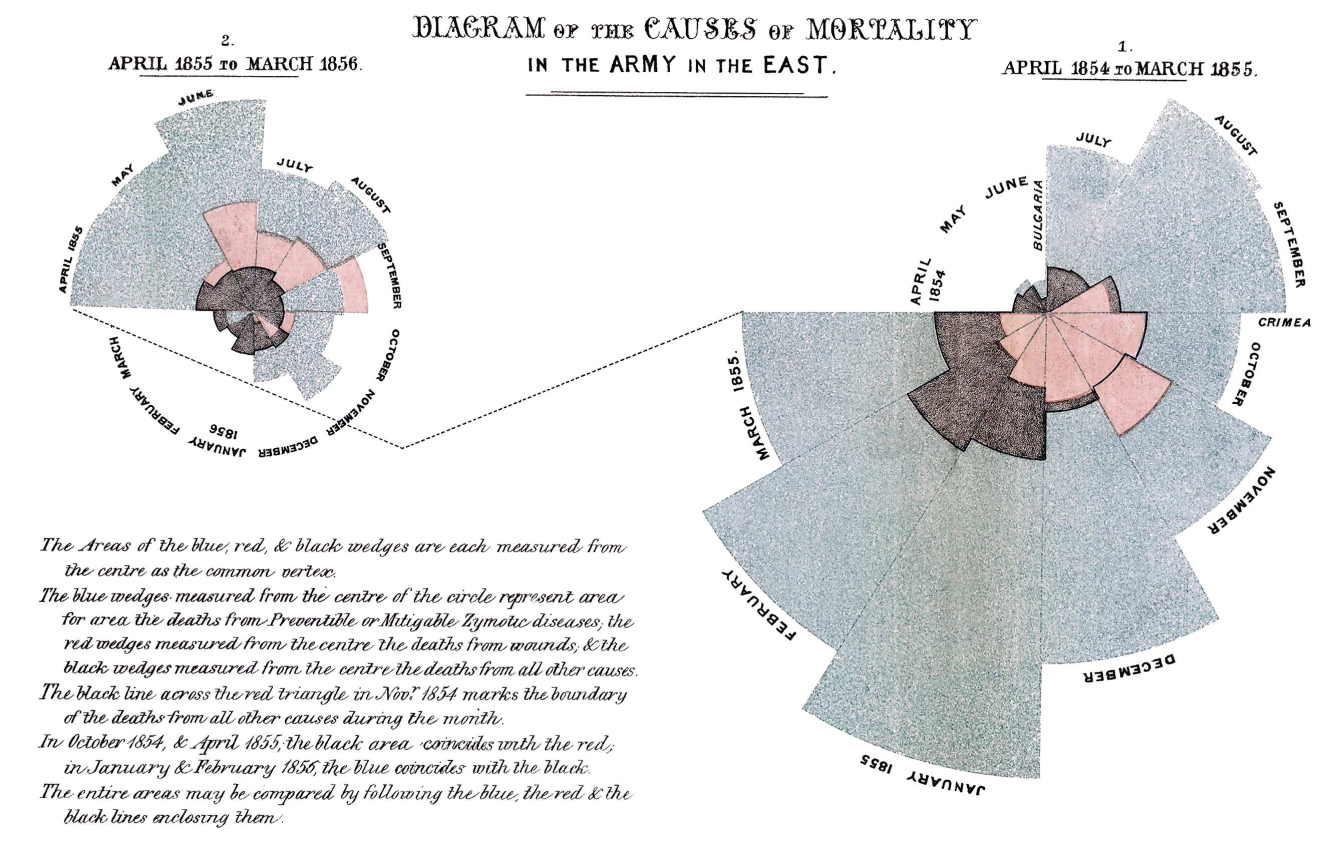
\includegraphics[scale=0.4]{figuras/rose-diagram.png}
\caption{O diagrama polar de Florence Nightingale (1854). Disponível em: \url{http://bit.ly/2MBkXkk}.}
\end{figure}
\end{minipage}
\end{frame}

% ----------------- NOVO SLIDE --------------------------------
\begin{frame}{Uma citação}
Relictum esse inspiratori Gombrich: 
\begin{quotation}
	``(...)Nam dui ligula, fringilla a, euismod sodales, sollicitudin vel, wisi. Morbi auctor lorem non justo. Nam lacus libero, pretium at, lobortis vitae, ultricies et, tellus. Donec aliquet, tortor sed accumsan bibendum, erat ligula aliquet magna, vitae ornare odio metus a mi. Morbi ac orci et nisl hendrerit mollis. Suspendisse ut massa. Cras nec ante. Pellentesque a nulla. Cum sociis natoque penatibus et magnis dis parturient montes, nascetur ridiculus mus. Aliquam tincidunt urna.(...)''\cite{gombrich} 
\end{quotation}

\end{frame}
% ----------------- NOVO SLIDE --------------------------------

% ----------------- NOVO SLIDE --------------------------------
\section{Um desenvolvimento}

\begin{frame}{Apenas um texto}
Lorem ipsum dolor sit amet, consectetuer adipiscing elit. Ut purus elit, vestibulum ut, placerat ac, adipiscing vitae, felis. Curabitur dictum gravida mauris. Nam arcu libero, nonummy eget, consectetuer id, vulputate a, magna. Donec vehicula augue eu neque. Pellentesque habitant morbi tristique senectus et netus et malesuada fames ac turpis egestas. Mauris ut leo, expressio \eqref{equationiae}: 
\begin{equation}
\int_{0}^{\infty} e^{x^{2}}dx = \frac{1}{2}\sqrt{\pi} \,.
\label{equationiae}
\end{equation}

\end{frame}
% ----------------- NOVO SLIDE --------------------------------
\begin{frame}{Uma tabela}
Conforme a tabela \ref{tabela:001}:
\begin{table}[]
	\caption{Para gerar tabelas em a partir de uma planilha, consultar \url{https://tablesgenerator.com/}.}
	\label{tabela:001}
	\begin{tabular}{|l|c|c|c|c|}
		\hline
		& \multicolumn{4}{c|}{Período de análise} \\ \hline
		Fluxo   & fev      & mar      & abr     & mai     \\ \hline
		Despesa &    1     &  2       &  3      &  4      \\ \hline
		Receita &    4     &  3       &  2      &  1      \\ \hline
	\end{tabular}
\end{table}
\end{frame}

\section{Considerações finais}

%% ----------------- NOVO SLIDE --------------------------------
\begin{frame}{Conclusiones}
\framesubtitle{Uma conclusão interessante}
A figura \ref{fig:grafxxx} ilustra a ideia.
\begin{figure}[hbtp]
	\centering
	
\includegraphics[scale=0.3]{figuras/abntex2-modelo-img-grafico.pdf}
	\caption{Veja que no Beamer não exibe o número da figura na legenda. Se quiser desenhar gráficos vetoriais, uma alternativa é o Inkscape: Disponível em: \url{https://inkscape.org/pt-br/}.} 
	\label{fig:grafxxx} 
\end{figure}
\end{frame}
%% ----------------- NOVO SLIDE --------------------------------

% ----------------- NOVO SLIDE --------------------------------
\begin{frame}{Considerações finais}
\framesubtitle{Etapas e/ou possíveis trabalhos futuros}
\begin{itemize}
	\item[\grimace] Publicação em periódicos; 
	\item[\textthing] Defesa;
	\item[\bomb] Escrita de um romance histórico;
	\item Um item menos ousado. 
\end{itemize}
\end{frame}
% ----------------- NOVO SLIDE --------------------------------

%\section{Referências}
% --- O comando \allowframebreaks ---
% Se o conteúdo não se encaixa em um quadro, a opção allowframebreaks instrui 
% beamer para quebrá-lo automaticamente entre dois ou mais quadros,
% mantendo o frametitle do primeiro quadro (dado como argumento) e acrescentando 
% um número romano ou algo parecido na continuação.

\begin{frame}[allowframebreaks]{Referências}
\printbibliography
\end{frame}

% ----------------- FIM DO DOCUMENTO -----------------------------------------
\end{document}